\documentclass[]{article}
\usepackage{lmodern}
\usepackage{amssymb,amsmath}
\usepackage{ifxetex,ifluatex}
\usepackage{fixltx2e} % provides \textsubscript
\ifnum 0\ifxetex 1\fi\ifluatex 1\fi=0 % if pdftex
  \usepackage[T1]{fontenc}
  \usepackage[utf8]{inputenc}
\else % if luatex or xelatex
  \ifxetex
    \usepackage{mathspec}
  \else
    \usepackage{fontspec}
  \fi
  \defaultfontfeatures{Ligatures=TeX,Scale=MatchLowercase}
\fi
% use upquote if available, for straight quotes in verbatim environments
\IfFileExists{upquote.sty}{\usepackage{upquote}}{}
% use microtype if available
\IfFileExists{microtype.sty}{%
\usepackage{microtype}
\UseMicrotypeSet[protrusion]{basicmath} % disable protrusion for tt fonts
}{}
\usepackage[margin=1in]{geometry}
\usepackage{hyperref}
\hypersetup{unicode=true,
            pdftitle={Progress Report},
            pdfauthor={Kiernan Nicholls},
            pdfborder={0 0 0},
            breaklinks=true}
\urlstyle{same}  % don't use monospace font for urls
\usepackage{longtable,booktabs}
\usepackage{graphicx,grffile}
\makeatletter
\def\maxwidth{\ifdim\Gin@nat@width>\linewidth\linewidth\else\Gin@nat@width\fi}
\def\maxheight{\ifdim\Gin@nat@height>\textheight\textheight\else\Gin@nat@height\fi}
\makeatother
% Scale images if necessary, so that they will not overflow the page
% margins by default, and it is still possible to overwrite the defaults
% using explicit options in \includegraphics[width, height, ...]{}
\setkeys{Gin}{width=\maxwidth,height=\maxheight,keepaspectratio}
\IfFileExists{parskip.sty}{%
\usepackage{parskip}
}{% else
\setlength{\parindent}{0pt}
\setlength{\parskip}{6pt plus 2pt minus 1pt}
}
\setlength{\emergencystretch}{3em}  % prevent overfull lines
\providecommand{\tightlist}{%
  \setlength{\itemsep}{0pt}\setlength{\parskip}{0pt}}
\setcounter{secnumdepth}{0}
% Redefines (sub)paragraphs to behave more like sections
\ifx\paragraph\undefined\else
\let\oldparagraph\paragraph
\renewcommand{\paragraph}[1]{\oldparagraph{#1}\mbox{}}
\fi
\ifx\subparagraph\undefined\else
\let\oldsubparagraph\subparagraph
\renewcommand{\subparagraph}[1]{\oldsubparagraph{#1}\mbox{}}
\fi

%%% Use protect on footnotes to avoid problems with footnotes in titles
\let\rmarkdownfootnote\footnote%
\def\footnote{\protect\rmarkdownfootnote}

%%% Change title format to be more compact
\usepackage{titling}

% Create subtitle command for use in maketitle
\newcommand{\subtitle}[1]{
  \posttitle{
    \begin{center}\large#1\end{center}
    }
}

\setlength{\droptitle}{-2em}

  \title{Progress Report}
    \pretitle{\vspace{\droptitle}\centering\huge}
  \posttitle{\par}
  \subtitle{GOVT-653}
  \author{Kiernan Nicholls}
    \preauthor{\centering\large\emph}
  \postauthor{\par}
      \predate{\centering\large\emph}
  \postdate{\par}
    \date{March 7, 2019}


\begin{document}
\maketitle

\subsection{Update}\label{update}

I have not made significant changes to the research question I initially
proposed. I am trying to determine the predictive capabilities of
markets as they compare to the more popular mathematical forecasting
models. Are prediction markets as accurate as forecasting models? Under
what conditions does each method perform? What role might prediction
markets play in the Congressional campaigns?

In statistical terms: I propose the null hypothesis of no difference in
proportion races correctly called by markets and models. Ultimately, I
hope to perform a test of equal proportion on a string of prediction
outcomes (correct or incorrect predictions).

\subsection{Market Data}\label{market-data}

PredictIt.org was launched in late 2014 to host prediction markets,
primarily on American politics. PredictIt is owned and operated by
\href{https://www.victoria.ac.nz/}{Victoria University of Wellington}
with support from \href{http://aristotle.com/}{Aristotle, Inc.}.
PredictIt partners with academic researchers, providing trading data for
research purposes. After signing a data use agreement with the site, the
provided me with trading data from 118 markets pertaining to 2018
Midterm elections.

The raw data spans 675 days from January 1, 2017 to December 12, 2018.
There are 44,711 observations of the following 11 variables:

\begin{enumerate}
\def\labelenumi{\arabic{enumi}.}
\tightlist
\item
  Market ID
\item
  Market question
\item
  Market symbol
\item
  Contract name
\item
  Contract symbol
\item
  Prediction date
\item
  Opening contract price
\item
  Low contract price
\item
  High contract price
\item
  Closing contract price
\item
  Volume of shares traded
\end{enumerate}

\begin{longtable}[]{@{}rlllrrr@{}}
\caption{10 of 44,711 observations with 7 of 11
variables}\tabularnewline
\toprule
ID & Market & Contract & Date & Open & Close & Volume\tabularnewline
\midrule
\endfirsthead
\toprule
ID & Market & Contract & Date & Open & Close & Volume\tabularnewline
\midrule
\endhead
4030 & CA39.2018 & GOP.CA39.2018 & 2018-02-26 & 0.31 & 0.31 &
0\tabularnewline
4255 & MN03.2018 & GOP.MN03.2018 & 2018-09-26 & 0.19 & 0.21 &
2\tabularnewline
3812 & AZSEN18 & DEM.AZSEN18 & 2017-11-16 & 0.48 & 0.57 &
41\tabularnewline
3532 & LEWI.MN02.2018 & n/a & 2018-05-09 & 0.36 & 0.36 &
0\tabularnewline
4271 & PA17.2018 & DEM.PA17.2018 & 2018-03-30 & 0.79 & 0.87 &
16\tabularnewline
2941 & MANCHIN.WVSENATE.2018 & n/a & 2018-04-09 & 0.73 & 0.70 &
116\tabularnewline
4156 & FL17.2018 & DEM.FL17.2018 & 2018-10-07 & 0.02 & 0.02 &
0\tabularnewline
3767 & NH01.2018 & DEM.NH01.2018 & 2018-06-12 & 0.83 & 0.83 &
0\tabularnewline
3503 & KING.MESENATE.2018 & n/a & 2017-11-06 & 0.87 & 0.87 &
0\tabularnewline
4257 & IL12.2018 & DEM.IL12.2018 & 2018-04-26 & 0.53 & 0.53 &
0\tabularnewline
\bottomrule
\end{longtable}

Each market poses a question (Which party will win the 2018 House of
Reps race in Texas's 21st district?). The possible answers to that
question (Democratic or Republican) are the contracts that comprise the
market. When a trader is interested in buying shares of a contract (100
shares of a Democratic party winning the Texas 21st for \$0.69 each),
they make an open offer on the market. A corresponding trader agrees to
buy the converse contract (100 shares of a Republican party winning the
Texas 21st for \$0.31 each). Those traders can buy or sell these shares
throughout the election at whatever price another trader agrees on.
After the election, each correct contract executes at \$1.00, with a
10\% fee going towards the operational costs of the exchange.

The price of a contract is directly proportional to the trader's
probabilistic interpretation of the election outcomes. If a trader
believes a party has a high chance of winning an election, he will not
place a bet without a low amount of risk. The binary outcome of the
futures contracts allow for a direct probabilistic interpretation of the
election results.

In market theory, the volume of shares traded plays a crucial role in
proper price discovery; too few shares traded and the market may not
properly react to changes in the election circumstances. In my analysis,
a market price over \$0.50 indicates a prediction of that candidate
winning the election. The closing price of a contract represents that
day's final market prediction. We can compare each day's prediction with
the eventual winner to assess the accuracy. The proportion of all races
correctly predicted represents the accuracy of the markets method.

\subsection{Model Data}\label{model-data}

FiveThirtyEight.com was launched in 2008 by Nate Silver to aggregate
polls of the Democratic Presidential Primary to better forecast the
winner. In the decade since, the model used by FiveThirtyEight has grown
in complexity. For the 2018 Midterm elections, FiveThirtyEight published
models for House, Senate, and Governors races. The models incorporate
quantitative inputs (primarily polling) to simulate the election and
produce a probabilistic view of the election.

The team at FiveThirtyEight makes public the top-line output of their
models as four separate \texttt{.csv} files on their website:

\begin{enumerate}
\def\labelenumi{\arabic{enumi}.}
\tightlist
\item
  \href{https://projects.fivethirtyeight.com/congress-model-2018/senate_national_forecast.csv}{\texttt{senate\_national\_forecast.csv}}
\item
  \href{https://projects.fivethirtyeight.com/congress-model-2018/senate_seat_forecast.csv}{\texttt{senate\_seat\_forecast.csv}}
\item
  \href{https://projects.fivethirtyeight.com/congress-model-2018/house_national_forecast.csv}{\texttt{house\_national\_forecast.csv}}
\item
  \href{https://projects.fivethirtyeight.com/congress-model-2018/house_district_forecast.csv}{\texttt{house\_district\_forecast.csv}}
\end{enumerate}

The Senate seat and House district level forecasts will be used in this
project. Each observation represents one day's probability of victory
for one candidate. There are 28,353 observations at the Senate seat
level and 302,859 at the House district level. Together, There are about
3,380 unique daily predictions from (97 days).

The raw data spans 97 days from August 1st to November 5th. Together,
the Senate and House data sets contain 328,113 observations of 12
variables:

\begin{enumerate}
\def\labelenumi{\arabic{enumi}.}
\tightlist
\item
  Prediction date
\item
  Election state
\item
  Election Congressional district
\item
  Whether the election is a ``special election''
\item
  Candidate's full name
\item
  Candidate's political party
\item
  Whether the candidate is an incumbent
\item
  Model version (classic, lite, or deluxe)
\item
  Candidate's probability of victory
\item
  Candidate's expected share of the vote
\item
  Candidate's approx. minimum share of the vote
\item
  Candidate's approx. maximum share of the vote
\end{enumerate}

\begin{longtable}[]{@{}llrllllrr@{}}
\caption{10 of 299,760 observations with 9 of 12
variables}\tabularnewline
\toprule
Date & State & District & Special & Party & Incumbent & Model & Win
Probability & Expected Share\tabularnewline
\midrule
\endfirsthead
\toprule
Date & State & District & Special & Party & Incumbent & Model & Win
Probability & Expected Share\tabularnewline
\midrule
\endhead
2018-10-01 & MD & 4 & NA & R & FALSE & deluxe & 0.000 &
18.67\tabularnewline
2018-10-08 & NC & 7 & NA & R & TRUE & lite & 0.778 &
52.06\tabularnewline
2018-08-20 & MI & 6 & NA & R & TRUE & deluxe & 0.892 &
53.47\tabularnewline
2018-08-13 & CA & 11 & NA & D & TRUE & deluxe & 1.000 &
77.44\tabularnewline
2018-10-26 & GA & 10 & NA & R & TRUE & deluxe & 1.000 &
67.81\tabularnewline
2018-10-19 & AL & 7 & NA & D & TRUE & lite & 1.000 &
100.00\tabularnewline
2018-09-05 & TX & 8 & NA & R & TRUE & deluxe & 1.000 &
75.15\tabularnewline
2018-08-04 & TX & 11 & NA & LIB & FALSE & deluxe & 0.000 &
3.31\tabularnewline
2018-09-28 & TX & 7 & NA & D & FALSE & classic & 0.480 &
49.80\tabularnewline
2018-09-18 & SC & 7 & NA & D & FALSE & lite & 0.036 &
39.82\tabularnewline
\bottomrule
\end{longtable}

\subsection{Tidy Data}\label{tidy-data}

The data from the markets and model can be combined and cleaned to
produce a single data frame with 26,778 observations of 10 variables:

\begin{enumerate}
\def\labelenumi{\arabic{enumi}.}
\tightlist
\item
  Prediction date
\item
  Election code
\item
  Candidate's name
\item
  Election chamber
\item
  Candidate's party
\item
  Whether the election is a ``special election''
\item
  Whether the candidate is an incumbent
\item
  Whether the prediction comes from the markets or model
\item
  Candidate's probability of victory
\end{enumerate}

\begin{longtable}[]{@{}llllllllr@{}}
\caption{10 of 26,778 observations with 9 variables}\tabularnewline
\toprule
Date & Race & Name & Chamber & Party & Special & Incumbent & Method &
Probability\tabularnewline
\midrule
\endfirsthead
\toprule
Date & Race & Name & Chamber & Party & Special & Incumbent & Method &
Probability\tabularnewline
\midrule
\endhead
2018-09-26 & CT-05 & Hayes & house & D & FALSE & FALSE & market &
0.950\tabularnewline
2018-08-09 & NC-13 & Manning & house & D & FALSE & FALSE & market &
0.550\tabularnewline
2018-08-09 & NY-01 & Zeldin & house & R & FALSE & TRUE & market &
0.710\tabularnewline
2018-10-17 & CA-10 & Denham & house & R & FALSE & TRUE & market &
0.290\tabularnewline
2018-08-27 & MA-99 & Warren & senate & D & FALSE & TRUE & model &
0.999\tabularnewline
2018-09-02 & NV-03 & Lee & house & D & FALSE & FALSE & model &
0.687\tabularnewline
2018-09-25 & MD-06 & Trone & house & D & FALSE & FALSE & market &
0.990\tabularnewline
2018-10-27 & IA-01 & Blum & house & R & FALSE & TRUE & model &
0.034\tabularnewline
2018-08-23 & PA-15 & Boser & house & D & FALSE & FALSE & market &
0.040\tabularnewline
2018-09-23 & VA-06 & Cline & house & R & FALSE & FALSE & market &
0.920\tabularnewline
\bottomrule
\end{longtable}

\subsection{Exploratory Plots}\label{exploratory-plots}

Below is a preliminary comparison of of each method's percentage of
correct predictions over time. More work needs to be done to properly
account for all the differences in the 111 races.

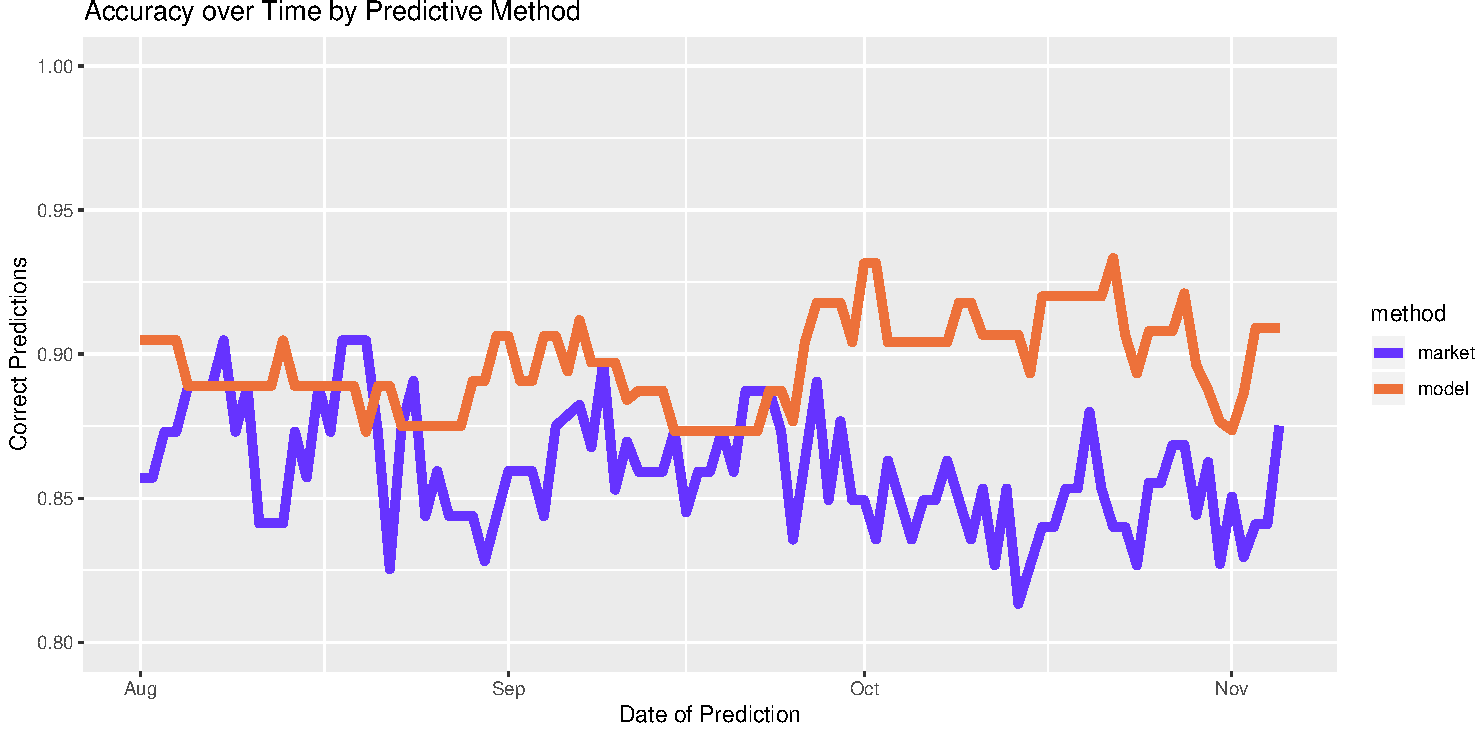
\includegraphics{progress_report_files/figure-latex/p2_plot-1.pdf}

Below are histograms comparing the distribution of probabilities in the
raw data sets from PredictIt and FiveThirtyEight the day before the
election. Note how the model predicts every race every day while the
markets only focus on races of interest to the traders. The races of
interest are those where the traders believe they can make a successful
bet against the market, meaning a greater proportion of the races
predicted by markets are toss-ups. Both methods will have to be assessed
on these shared races of interest.

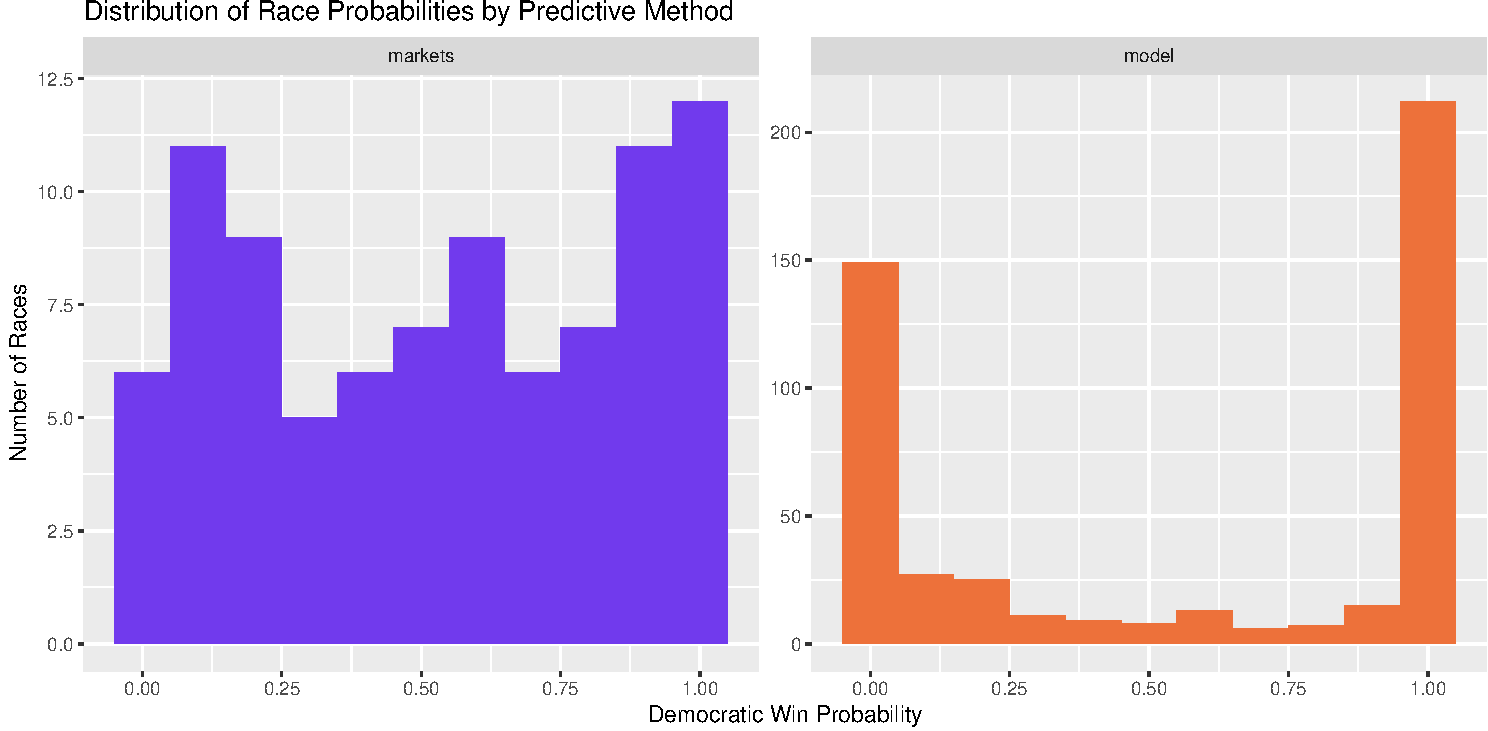
\includegraphics{progress_report_files/figure-latex/plot_races_hist-1.pdf}

Another point of difference is the number of predictions made by each
method over time. The model model predicts every race every day, whereas
more markets are added to the exchange every day. Below is a plot
showing the number of open midterm election markets hosted on the
PredictIt exchange in 2018.

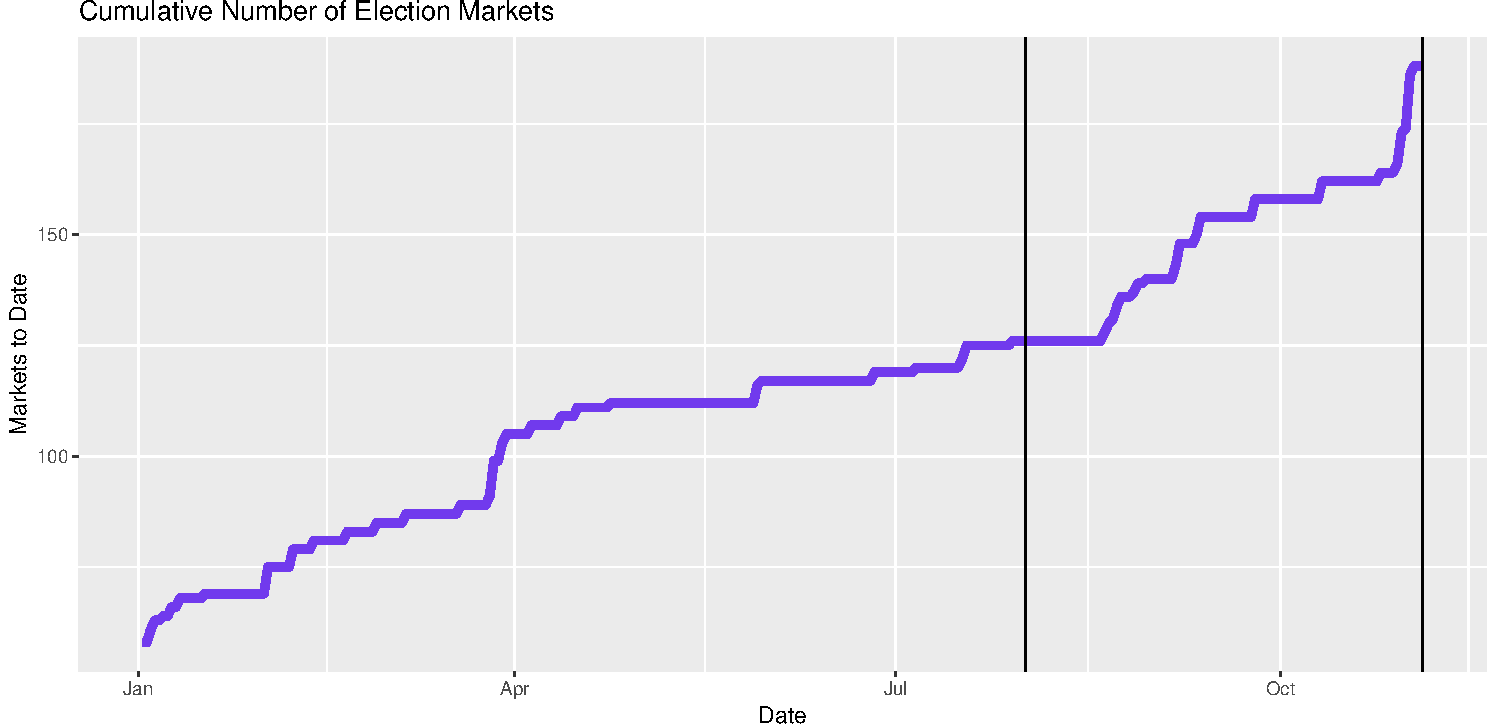
\includegraphics{progress_report_files/figure-latex/plot_cum_markets-1.pdf}

Below are plots showing the the increase in the two underlying inputs in
each method. While the model takes into account a number of quantitative
factors, polling still plays the largest and more useful roll in
predicting an election. Similarly, the accuracy of prediction markets
relies on the volume of the markets; the greater the volume of money
being exchanged on the markets, the greater the economic forces of price
discovery and can capture the underlying probabilities associated with
the market equilibrium.

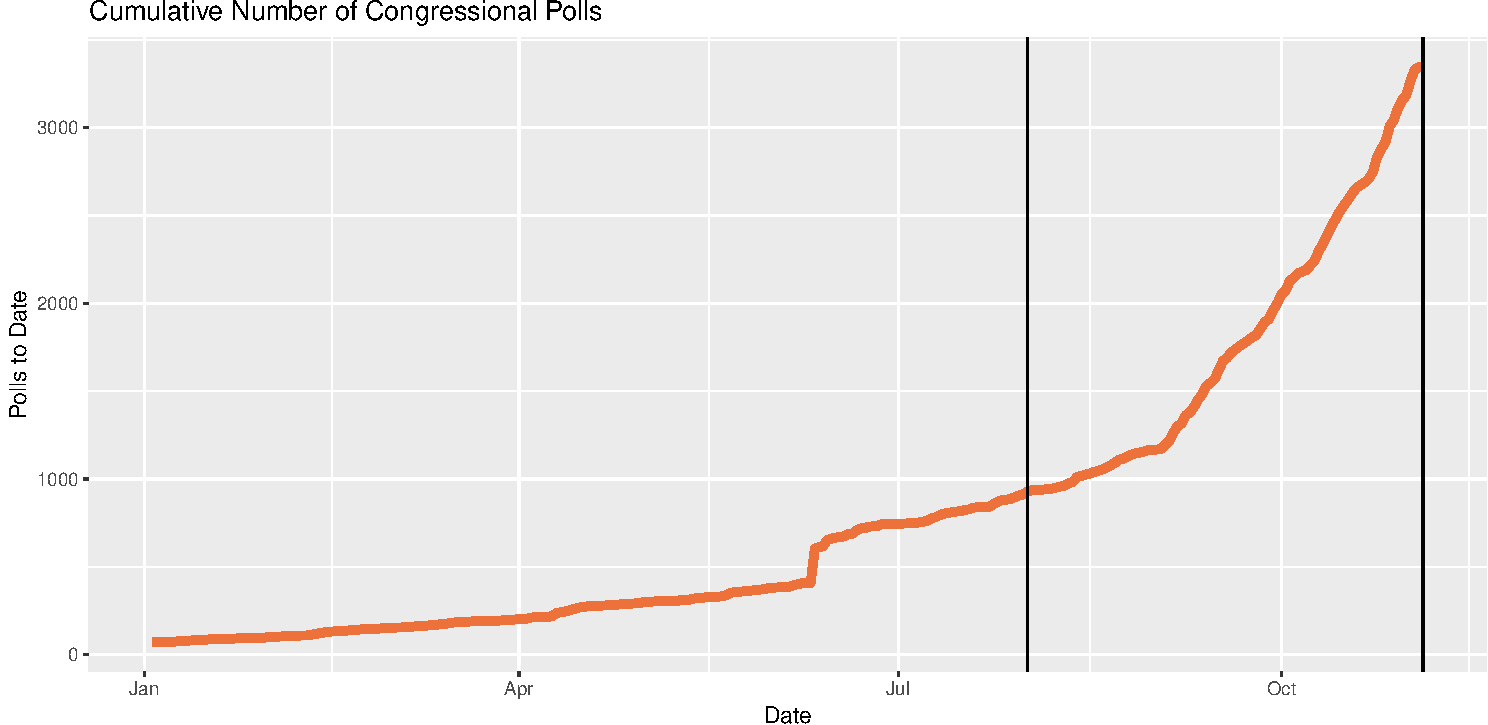
\includegraphics{progress_report_files/figure-latex/plot_cum_polls-1.pdf}
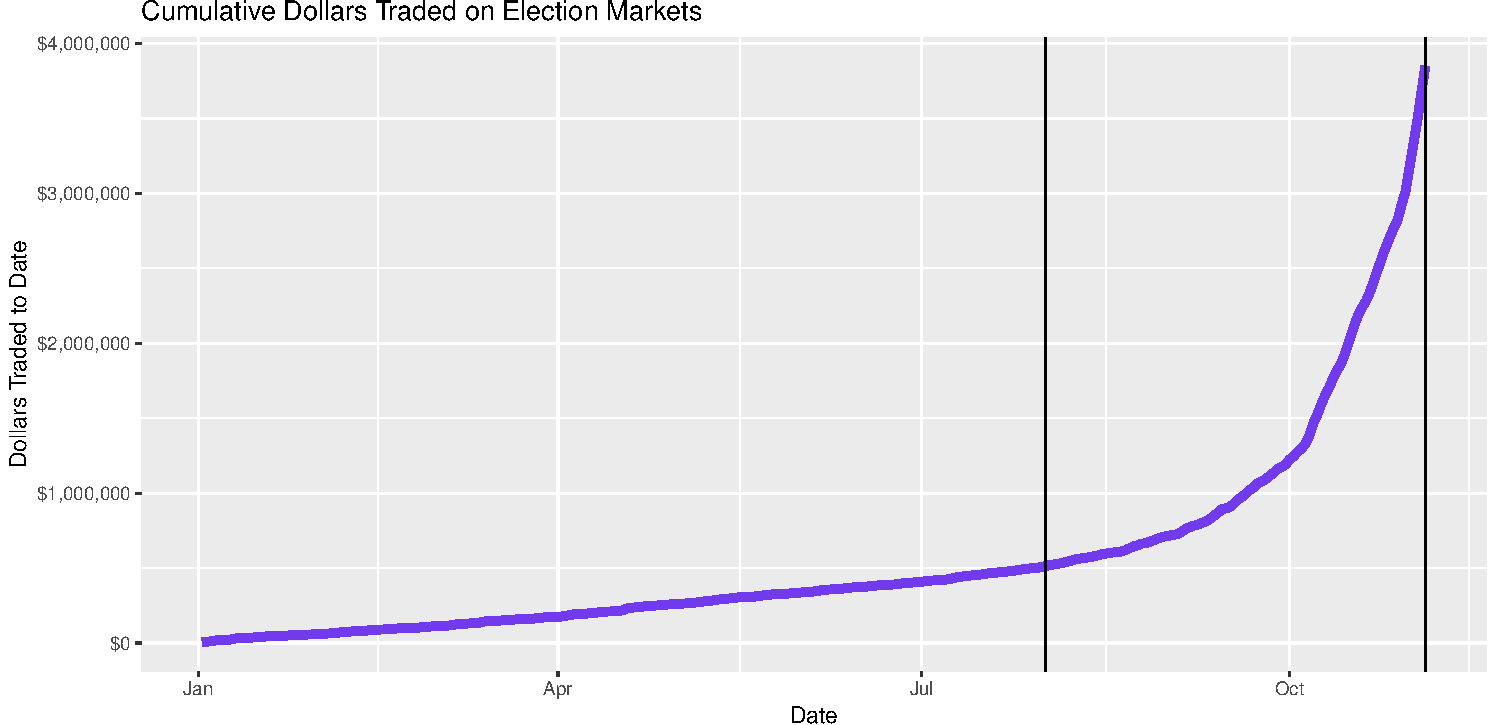
\includegraphics{progress_report_files/figure-latex/plot_cum_polls-2.pdf}


\end{document}
